\documentclass[preprint]{iacrtrans}

\usepackage[utf8]{inputenc}
\usepackage{amssymb, amsmath, amsfonts, amscd}
\usepackage[T1]{fontenc}
\usepackage{graphicx}
\usepackage{url}
\usepackage{xspace}
\usepackage{subcaption}
\usepackage{algorithm2e}
\usepackage{tikz}
\usepackage{cellspace}
\usepackage{multirow}
%\usepackage{parskip}
\usetikzlibrary{patterns}

%\usepackage[noend]{algpseudocode}

\usepackage[pdftex,bookmarks,bookmarksopen,bookmarksdepth=3]{hyperref}
\hypersetup{colorlinks=true,citecolor=red,linkcolor=red,urlcolor=black}

\usepackage{algorithmic}

% knuth-style algos
\newcommand{\slug}{\hbox{\kern1.5pt\vrule width2.5pt height6pt depth1.5pt\kern1.5pt}}
\def\xskip{\hskip 7pt plus 3pt minus 4pt}
\newdimen\algindent
\newif\ifitempar \itempartrue % normally true unless briefly set false
\def\algindentset#1{\setbox0\hbox{{\bf #1.\kern.25em}}\algindent=\wd0\relax}
\def\algbegin #1 #2{\algindentset{#21}\alg #1 #2} % when steps all have 1 digit
\def\aalgbegin #1 #2{\algindentset{#211}\alg #1 #2} % when 10 or more steps
\def\aaalgbegin #1 #2{\algindentset{#2111}\alg #1 #2} % when 10 or more steps
\def\alg#1(#2). {\medbreak % Usage: \algbegin Algorithm A (algname). This...
  \noindent{\bf#1}({\it#2\/}).\xskip\ignorespaces}
\def\algstep#1.{\ifitempar\smallskip\noindent\else\itempartrue
  \hskip-\parindent\fi
  \hbox to\algindent{\bf\hfil #1.\kern.25em}%
  \hangindent=\algindent\hangafter=1\ignorespaces}
% end of borrowed macros

\newcommand{\todo}[1]{\textcolor{red}{TODO:[#1]}}

\title{Predicting the PCG PSeudo-Random Number Generator In Practice} 

\author{Charles Bouillaguet\inst{1} \and Julia Sauvage\inst{2} \and Florette Martinez\inst{3}}


\institute{% 
University of Lille, France \\ 
\email{charles.bouillaguet@univ-lille.fr}
\and 
Sorbonne University \\
\email{julia.sauvage@etu.upmc.fr}
\and 
LIP6, CNRS, SU ? \\
\email{florette.martinez@lip6.fr}

}

\begin{document}
\maketitle

\keywords{keywords}

\begin{abstract}
  blablabla
\end{abstract}

\section{Introduction} %ce qu'on avait écrit pour le projet, peut-être pas incroyable...

\todo{Ca, c'est du blabla...}

Pseudo-random generators (PRG) are well-studied primitives in symmetric
cryptography. A PRG is an efficient deterministic algorithm that stretch a small
random seed into a longer pseudo-random stream. To achieve cryptographic-grade
pseudo-randomness, a PRG must ensure that the pseudo-random stream is
computationally indistinguishable from a ``truly'' random sequence of bits by
efficient adversaries. Alternatively, it is possible to define pseudo-randomness
by asking that no efficient algorithm is capable of predicting the next
pseudo-random bit with non-negligible accuracy. The two definitions are in fact
equivalent.

\todo{mentioner stream ciphers}

Not all pseudo-random generators are of cryptographic strength. In some
applications, it is not necessarily necessary: to be used in Monte-Carlo
simulations or generate random choices in games, a relaxed, non-cryptographic
notion of pseudo-randomness may be sufficient. This allows for faster
algorithms. For instance, the \texttt{Math.Random} function in Google's V8
open-source JavaScript engine uses the \textsf{XorShift128} generator, which is
a Linear Feedback Shift Register tailored for high software speed. On 64-bit
processors, it produces 64 pseudo-random bits with 3 shifts and 4 XORs
instructions. The \textsf{python} standard library's \texttt{random} module uses
the Mersenne Twister. The \textsf{C} library that comes along \texttt{gcc} (the
\texttt{glibc}) uses a (poor) truncated linear congruential generator by default
to implement the \texttt{rand} function.

In the realm of non-cryptographic random generators, a PRG is deemed ``good
enough'' it is passes \emph{some} efficient statistical tests --- whereas the
cryptographic notion of pseudo-randomness asks that it passes \emph{any}
efficient test. There are \textit{de facto} statistical test suites (\todo{les
  mentionner}). The goal of designers then consists in designing the fastest
possible generator that passes the day's favorite test suite.

\todo{Mentionner Ferrenberg 92}

The scientific computing community also realized that the need for fast
\emph{parallel} random number generation could be satisfied by the use of block
ciphers in counter mode~\cite{Salmon11}. The need for speed then leads to the
use of weakened cryptographic primitives.

In most cases, it is easy to see that a non-cryptographic PRG does not meet the
cryptographic notion of pseudo-randomness, and there are few exceptions. In this
paper, we study the \textsf{PCG} family of non-cryptographic pseudo-random
generators~\cite{melissapaper,melissaweb}.

\textsf{PCG} stands for ``Permuted Congruential Generator'': it essentially
consists in applying a non-linear filtering function on top of a (fairly weak)
linear congruential generator (in a way reminiscent to the venerable filtered
LFSRs). The resulting combination is fast and passes current test suites. Its
designer claimed that distinguishing the pseudo-random stream produced would be
``challenging''. The \textsf{PCG} family contains many members, but we focus on
its strongest member, named either \textsf{PCG64} or \textsf{PCG-XSL-RR}. It has
a 128-bit internal state and produces 64 bits when clocked. It is the default
pseudo-random number generator in the popular \textsf{NumPy} scientific
computing package for \textsf{Python}.

The internal state of the \textsf{PCG64} generator is made of a 128-bit
``state'' and a 128-bit ``increment'', whose intended use is to provide several
pseudo-random streams with the same seed (just as the initialization vectors do
in stream ciphers). A default increment is provided in case the end-user just
want one pseudo-random stream with a single 128-bit seed.

\paragraph{Contribution.} We describe an algorithm that reconstructs the full
internal state of the strongest member of the \textsf{PCG} family. This allows
to predict the pseudo-random stream deterministically and clock the generator
backwards. The original seeds can also easily be reconstructed. The algorithm is
practical and we have executed it in practice. It follows that predicting the
output of the \textsf{PCG} should not be considered challenging anymore.

Our algorithm reconstruct the internal state using the ``guess-and-determine''
technique: some bits of the internal state are guessed ; assuming the guesses
are correct, some other information is computed ; a consistency check discards
bad guesses early on ; then candidate internal states are computed and fully
tested. The problem actually come in two distinct flavors.

When the increment is known (for instance when it is the default value), a
simplified prediction algorithm recovers the internal state from 192 bits of
pseudo-random stream. The process runs in 20 CPU minutes (on a single core of a
server processor). It guesses 36 bits of the internal state, then solves an
instance of the \textsc{Closest Vector Problem} (CVP) in a 3-dimensional
euclidean lattice. This requires about 50 arithmetic operations in total and
reveals the entire internal state if the guesses are correct.

When the increment is unknown, things are a bit more complicated. This is the
default situation in \textsf{NumPy}, where both the state and the increment are
initialized using an external source of entropy. In this case, our prediction
algorithm requires 3072 bits of pseudo-random stream ; it guesses between 51 and
55 bits, then for each guess it solves and instance of CVP in dimension 4 (using
about 75 arithmetic operations). This recovers 64 more bits of information about
the difference between two successive states, and this is enough to filter the
bad guesses. This information can then be used in a subsequent and comparably
inexpensive phase to recover the entire internal state. On average, the whole
process requires a bit less than 20 000 CPU hours to complete.

We implemented the algorithms in \textsf{C}, then asked the designer of the PCG
family to send us ``challenge'' pseudo-random streams ; we ran our code and
emailed back the seeds used to generate the challenge streams the next day.

\paragraph{Related Work.} \todo{Mentionner Knuth et les LCG + Frieze + Boyar + Stern...}

\todo{mentionner Vigna ?}

% The combination between being highly commended (it achieved 5th place out of 29
% in a recent performance test survey\cite{survey}) and a well presented
% website\cite{melissaweb} giving an feeling of professionalism can lead to the
% impression that PCG is a sufficiently secure family of generators.

% Some attacks against PCG have been carried out by Sebastiano
% Vigna\cite{vignaweb}, but this didn't yield any significant results, given that
% he only tried to break an incomplete version in a fairly straightforward way. He
% worked on a very specific version of PCG. He considers the result without
% modulo, which is a big simplification. Moreover, he didn't study the 128 bits
% long generator, but only the 64 bits long\cite{vignacode}.


\section{The PCG Pseudo-Random Number Generator Family}

\todo{cette section doit décrire précisément PCG.}

\begin{quote}
  In addition, one of the generators, PCG-XSL-RR(described in Section 6.3.3), is
  explicitly designed to make any attempt at state reconstruction especially
  difficult, using xor folding tominimize the amount of information about
  internal state that leaks out.
\end{quote}

\begin{quote}
  Although these properties make it extremely challenging for an agent observing
  theexternal behavior of a program to guess the state of its random number
  generator,
\end{quote}

% import numpy
% print(numpy.random.default_rng())
% ---> Generator(PCG64)

\subsection{LCG algorithm}

The PCG algorithm we studied is based on the Linear Congruential Generators algorithm. The LCG algorithm is simply based on a congruential multiplication. This type of generator is based on four values: an internal state $S_{i}$, a multiplier $A$, an increment $C$ and the size $M$. Generally, to initialize a generator of a given size, a seed value is provided as the first internal state, and a default multiplier and increment are used. We will study the case where $M$ and $A$ are known and where $M$ is a power of 2.\\

Calling the generator results in calculating the next internal state $S_{i+1} = A \times S_i + C \mod{M}$ and outputting $S_{i+1}$ as data.

This type of generator is trivially predictable because, the internal state is given to us at each output, and in the event that $C$ is unknown, we can still deduce it with two consecutive outputs: $C = S_{i+1} - A \times S_i$.\\

A better variant of the standard LCG is the Truncated LCG, where the output consists only of the higher bits of the internal state $S_i$. This way the entire internal state isn't accessible. Returning the lower bits is not interesting because as we can understand easily and will prove later, lower bits of a state only depend on the lower bits of the previous state.

\subsection{PCG algorithm}

The PCG algorithm we studied is based on the LCG algorithm. To start, here are a few definitions:
\begin{itemize}
    \item let $k$ be the size of our generator, in this case $k = 128$ bits;
    \item let $M$ be the modulus with $M = 2^k$;
    \item let $S_i$ be the internal state at the $i$-th iteration and $S$ be the list of $S_i$;
    \item let $X_i$ be the output at the $i$-th iteration of the generator and $X$ be the list of $X_i$;
    \item let $lowS_i$ be the $k/2$ least significant bits of $S_i$;
    \item let $upS_i$ be the $k/2$ most significant bits of $S_i$;
    \item let $rot_i$ be the 6 most significant bits of $S_i$;
    \item let $nbiter$ be the number of consecutive outputs for prediction purposes.
\end{itemize}

The internal state can be redefined as:
\begin{equation}
    S_i = 2^{k/2} \times upS_i + lowS_i 
\end{equation}

The 6 most significant bits, $rot_i$, of the internal state are used as a value to determine the rotation in the PCG algorithm. Let \texttt{rotate} be the function that performs said rotation (Figure \ref{pcg128out}).\\
The rotation is a simple exchange of bits, where a $k/2$ bit value is split into 2 parts: one of $rot_i$ bits and the other in $(k/2) - rot_i$ bits. The two parts are then swapped, and the new value is returned. 

This generator is initialised with a given $k$ bit internal state $S_0$ (of size 128 bits in the case of PCG128), and optionally with an $k$ bit increment $C$. If no increment is given, the algorithm will use a known default increment. For each output of the generator, the algorithm will perform the following calculations" (Figure \ref{pcg128out}):\\
\begin{align}
    X_{i} &= \mathtt{rotate}(upS_i\ \mathtt{XOR}\ lowS_i)\\
    S_{i+1} &= A \times S_{i} + C \mod{2^k}
\end{align}
In the case of PCG128, $A$ is a default increment of size 125 bits prime with $2^k$.

\begin{figure}[h!]
    \centering
    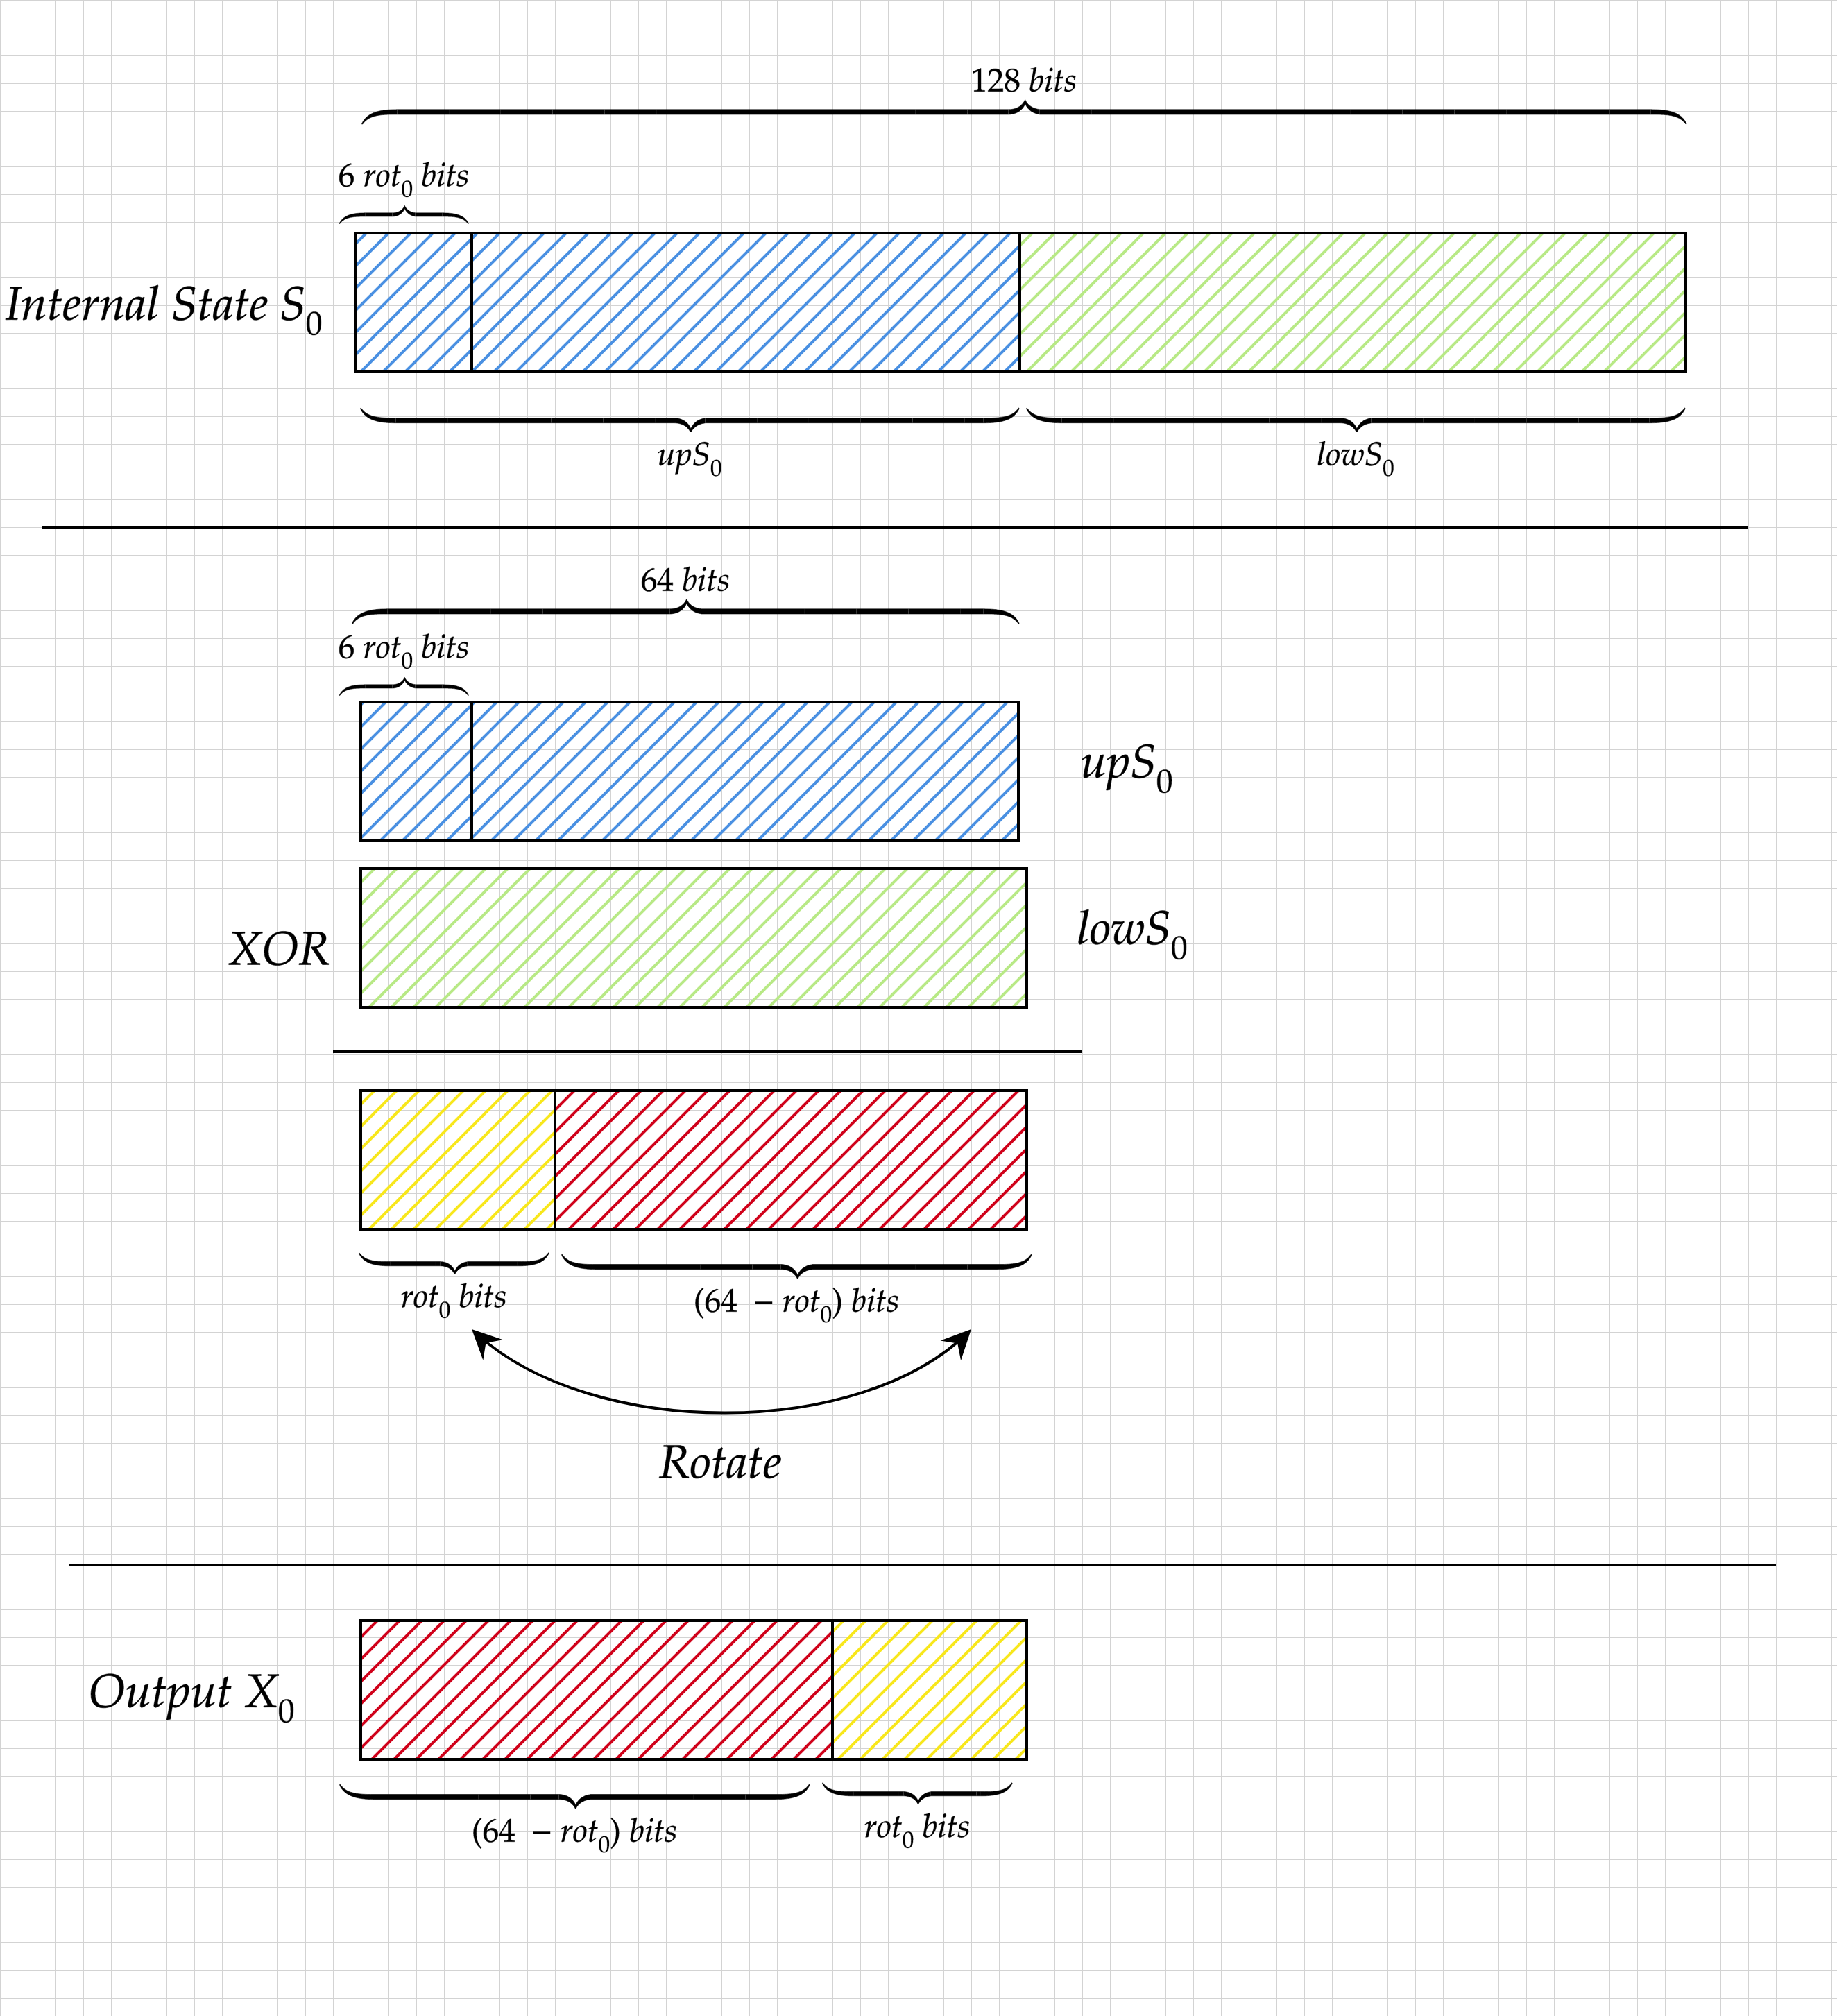
\includegraphics[width=0.75\linewidth]{pictures/PCG128.png}
    \caption{PCG128 : Output process}
    \label{pcg128out}
\end{figure}



Given the nature of the generator, the following values are known at every step:
\begin{itemize}
    \item the size of the generator $k$;
    \item the list of outputs $X$;
    \item the multiplier $A$;
    \item and eventually $C$, if the default increment was used. 
\end{itemize}

To break this generator, we had to differentiate between cases when the default $C$ was used or not. It was also interesting to note what was the minimum number of $X_i$ needed to reliably attack it.




\section{Naive Brute-Force Reconstruction of the Internal State}

In this section we describe the simplest possible prediction algorithm we could
think of. They serve as ``baseline'' to evaluate the more refined predictors
described below.

\todo{Dans le cas où C est connu, c'est le truc de Vigna, non ?}

\subsection{Brute-Force Attack with known $C$}

In the case where $C$ is known, if we find $S_0$, we can calculate every $S_i$
with the given formula, and predict all the following outputs of the
generator. The naive way is by doing a comprehensive research of $upS_0$, and
then calculating $lowS_0$ with the formula :
\begin{equation}
    lowS_0 = upS_0\ \mathtt{XOR}\ \mathtt{unrotate}(X_0)
\end{equation}
with \texttt {unrotate} being the inverse function of \texttt{rotate}.


If our guessing of $upS_0$ is correct, we can obtain the correct $X_1$ with
$S_1$ deduced from the initial $S_0$. The preceding is a naive method for
predicting PCG generator in $2^{64}$ operations. But we can have other values
that verify that test. This will not return $S_0$ but a very short list of
possibles $S_0$, with the actual one in it. We just need to test the following
outputs to find the real $S_0$. This is yet a very slow way to guess the
internal state, so we need a better solution.

\subsection{Brute-Force Attack with unknown $C$}

In case $C$ is unknown, retrieving $S_0$ is harder. The naive algorithm gives us
an answer within $2^{128+6}$ simple operations whit the following algorithm:

\begin{algorithmic}[!h]
\FOR{all possibilities of $lowC$ and $upS_0$}
    \STATE \texttt{unrotate}($X_0$)
    \STATE $lowS_0 = upS_0\ \mathtt{XOR}\ X_0$
    \STATE $lowS_1 = lowC + lowS_0 \times A \mod{2^{k/2}}$
    \FOR{all possibilities of $rot_1$}
        \STATE $\mathtt{unrotate}(X_1)$
        \STATE $upS_1 = lowS_1\ \mathtt{XOR}\ X_1$
        \STATE $C = S_1 - A \times S_0 \mod{2^{k}}$
        \STATE $S_2 = S_1 \times A + C$
        \IF {$S_2$ is coherent with  $X_2$}
            \STATE print($C$,$S_0$)
        \ENDIF
    \ENDFOR
\ENDFOR
\end{algorithmic}

This algorithm reveals us $C$ and a list of outputs with $S_0$ in it. The entry
is 256 bits long, and we used 3 64 bits long outputs of the generator. There
will be about $2^{64}$ possible $S_0$. This is why we need a couple other
outputs to get the real $S_0$. Sorting out which is the correct $S_0$ can be
done afterwards, and won't affect the complexity. But given the complexity of
this algorithm, it is even more unrealistic to solve problem in this fashion
then the previous one where $C$ was known.


\section{Predicting Truncated Linear Congruential Generators}

\todo{Comme on utilise à plusieurs reprise l'idée de se ramener à un LCG
  tronqué, autant décrire la technique à base de réseaux un bon coup.}

The algorithm of Frieze \textit{et al}\cite{Frieze} solves the case where $M$
and $A$ are known, $M$ being a power of two and, possibly with a significant
portion of the internal state unknown. The known part is the upper bits of the
state. This algorithm is coherent with our problem, this being the reason why we
focused on this one in particular. However, this algorithm won't work for some
particular multipliers. But this problem doesn't concern us, because the default
multiplier of \texttt{PCG128} is not one of them.

The first article we found was written by Joan Boyar\cite{Boyar1989}. The
subject of her study was a special case of truncated LCG, with $A$, $C$ and $M$
unknown and has access to a very large part of the internal state. This made it
so that we couldn't use her findings, because guessing a large part of the
internal state wouldn't be cost-effective. However, her study included a very
broad state of the art, explaining the specifics of many algorithms, as well as
describing in which circumstances they should be used.


%\subsection{Different solutions for Truncated Linear Congruential Algorithms}

\subsection{Frieze \textit{et al} algorithm}

The algorithm we studied uses lattices, and more specifically use the\break Lenstra–Lenstra–Lovász lattice basis reduction algorithm (LLL algorithm)\cite{LLLpastack}. A large part of this algorithm is very well explained on Stack Overflow\cite{LLLstack}.
We will detail the entire algorithm here.\\

A lattice in $\mathbb{R}^n$ is a subgroup of the additive group $(\mathbb{R}^n,+)$, isomorphic to $(\mathbb{Z}^n,+)$. The LLL algorithm is an approximation algorithm of the reduction of a lattice basis. It returns a reduced basis, with shorter vectors than the ones given. These vectors are a good approximation of the basis with the smallest determinant.\\

To use this algorithm, we reduce the sequence of $S_i$ to a geometric sequence $S'$ and, given the relationship between $S$ and $S'$, we can retrieve $S$. There are different methods to achieve this result and we selected two of them in our optimised algorithms. Consider the following geometric sequence:
\begin{equation}
    S'_i=\alpha ^i \times S'_0 \mod{M}
\end{equation}
With $S'$ as the vector made of all the $S'_i$ of length $nbiter$, and $A$ blocked, the $S'$ vectors are the vectors of the lattice generated by the matrix :

\begin{equation}
L=
\begin{pmatrix} 
M & 0 & & \dots & 0\\
\alpha & -1 & 0 & \dots & 0\\
\alpha ^2 & 0 & -1 & \dots & 0\\
\vdots & & & \ddots & \vdots\\
\alpha ^{nbiter - 1} & 0 & 0 & \dots & -1
\end{pmatrix}
\end{equation}

%Beau "ell" : $\ell$

Let $Y$ be the most significant bits of the internal states of LCG, and $Z$ be the lower bits, with $S = Y + Z$. We already know $Y$ from the outputs and we are searching for $Z$. 
\begin{itemize}
    \item Let $Y'$ be the upper bits of $S'$;
    \item Let $Z'$ be the lower bits;
    \item Let $L'$  be the reduced matrix returned by the LLL algorithm for $L$ ($L' = LLL(L)$);
\end{itemize}

By definition of $L$, we have :
\begin{align}
    L \times S' &=0 \mod{M}\\
    L' \times S' &= 0 \mod{M}\\
    L' \times (Y' + Z') &= M \times \ell\ \text{($\ell$ unknown integer vector)}\\
    L' \times Z' &= M \times \ell - L' \times Y'
\end{align}
We have $M = 2^k$. L' coefficients are small. We want to find the actual value of $\ell$.\\

We suppose we have every coordinate of $L' \times Z'$ smaller than $M/2$. Then every coordinate of $M \times \ell - L' \times Y'$ is smaller than $M/2$ and $M \times \ell$ is the closest vector of $M$ multiples from $L' \times Z'$. We have $\ell$ is the closest integer vector from $(B \times y)/M$.\\

The only unknown variable left is $Z'$ and :
\begin{equation}
    Z' = L'^{-1} \times (M \times k) - Y' 
\end{equation}
Now we know $Z'$, and the integer $S' \mod{M}$, and finally, $S \mod{M}$ the internal state we were looking for.\\

\subsection{Application to our generator}
The $L$ matrix for our problem is :
\begin{equation}
    L=
\begin{pmatrix}
1208925819614629174706176 & 0 &  0 &  0 &  0 &  0 &  0 &  0 &  0 & 0\\
442210214475561085761093 & -1 &  0 &  0 &  0 & 0 &  0 &  0 &  0 &  0\\
548907270092662740397721 & 0 & -1 &  0 &  0 & 0 &  0 &  0 &  0 &  0\\
68528166612430993102141 & 0 &  0 & -1 &  0 & 0 &  0 &  0 &  0 &  0\\
579003058182980434679665 & 0 &  0 &  0 & -1 & 0 &  0 &  0 &  0 &  0\\
907267876411637163239285 & 0 &  0 &  0 &  0 & -1 &  0 &  0 &  0 &  0\\
971193525585951128490121 & 0 &  0 &  0 &  0 & 0 & -1 &  0 &  0 &  0\\
423043601822819931331309 & 0 &  0 &  0 &  0 & 0 &  0 & -1 &  0 &  0\\
722352710310758831226849 & 0 &  0 &  0 &  0 & 0 &  0 &  0 & -1 &  0\\
239218985093571541740965 & 0 &  0 &  0 &  0 & 0 &  0 &  0 &  0 & -1
\end{pmatrix}
\end{equation}
Each coefficient is about 128 bit long. Here is the $L'$ (using the LLL algorithm of Sagemath \cite{sagemath}):
\begin{equation}
\begin{pmatrix}
    L' =
    77 & -105 & -115 &  17 & -108 & -77  & -7 &  50 & 107 &  17\\
     50  & 80 & 9 & -90 &  138 & -104  & 26  & 90 & -17 & -134\\
    14 & -42 & 130 & -67 & -31 & -172 & 122 & -76 & -32 &  14\\
    -61 &  97 &  70 & 161  & -4 & -229 & -23 & -44  & -1 & -26\\
    118  & 33 & -65 &  -3 &  83 & -176 & -187 & -70 &  25 &  34\\
    111 & -151 & -73 & 115 &  36 & 200 &  79  & -1 & -14 & -82\\
    94  & 15 & -18 & -36 & 142 & -47 &  32 & -188 & 161 & -127\\
    126 & -10 & 129 & 173 & -71  & 61 & -137 &  69 & 7 &  77\\
    174 & -62 &  58  & 39 &  79 & -133 &  93 & 115 &  24 & 181\\
    48 & 240 &  -2 & 114 & -15 &  37 & 145 & -100 &  24 & -19\\
\end{pmatrix}
\end{equation}
This algorithm is clearly really efficient, the coefficients of $L'$ are really small. Its bigger coefficient is $240$. Its smaller than $2^8 = 256$. In our case $M = 2^{64 + known\_low}$. In our tests, we had $known\_low = 16$. We need $Z'$ to be less than 72 bits long, which isn't hard to attain.

\section{Predicting PCG with Known Increment}
\subsection{Reduction to a truncated LCG model}
By exploiting the nature of this generator, it becomes apparent that some values can be easily guessed. We already saw that if we guess $rot_i$, then retrieving $X_i$ becomes a simple \texttt{XOR} operation, and in turn, if we have some knowledge of a particular bit of $lowS_i$ (respectively $upS_i$), we can deduce the equivalent bit from $upS_i$ (respectively $lowS_i$).\\

Moreover, there is an interesting proprity concerning the least significant bits of the internal state. Indeed, if we define $lowC$ as the 64 least significant bits of $C$ ($lowC = C \mod{2^{k/2}})$, we have:

\begin{align}
    S_{i+1} &= A \times S_i + C \mod{2^k}\\
    upS_{i+1} \times 2^{k/2} + lowS_{i+1} &= A \times upS_i \times 2^{k/2} + A \times lowS_i + C \mod{2^k} \\
    lowS_{i+1} &= A \times lowS_i + lowC \mod 2^{k/2}
\end{align}
We can see that $lowS_{i+1}$ is independent from $upS_i$. That mean that knowing $lowS_i$, we can deduce all $lowS_j$ with $j>i$. This relationship is used in the Brute-Force attack with known $C$, in the previous section.
We can see on (Figure \ref{pcg128goodbits})%figure
\begin{figure}[h!]
    \centering
    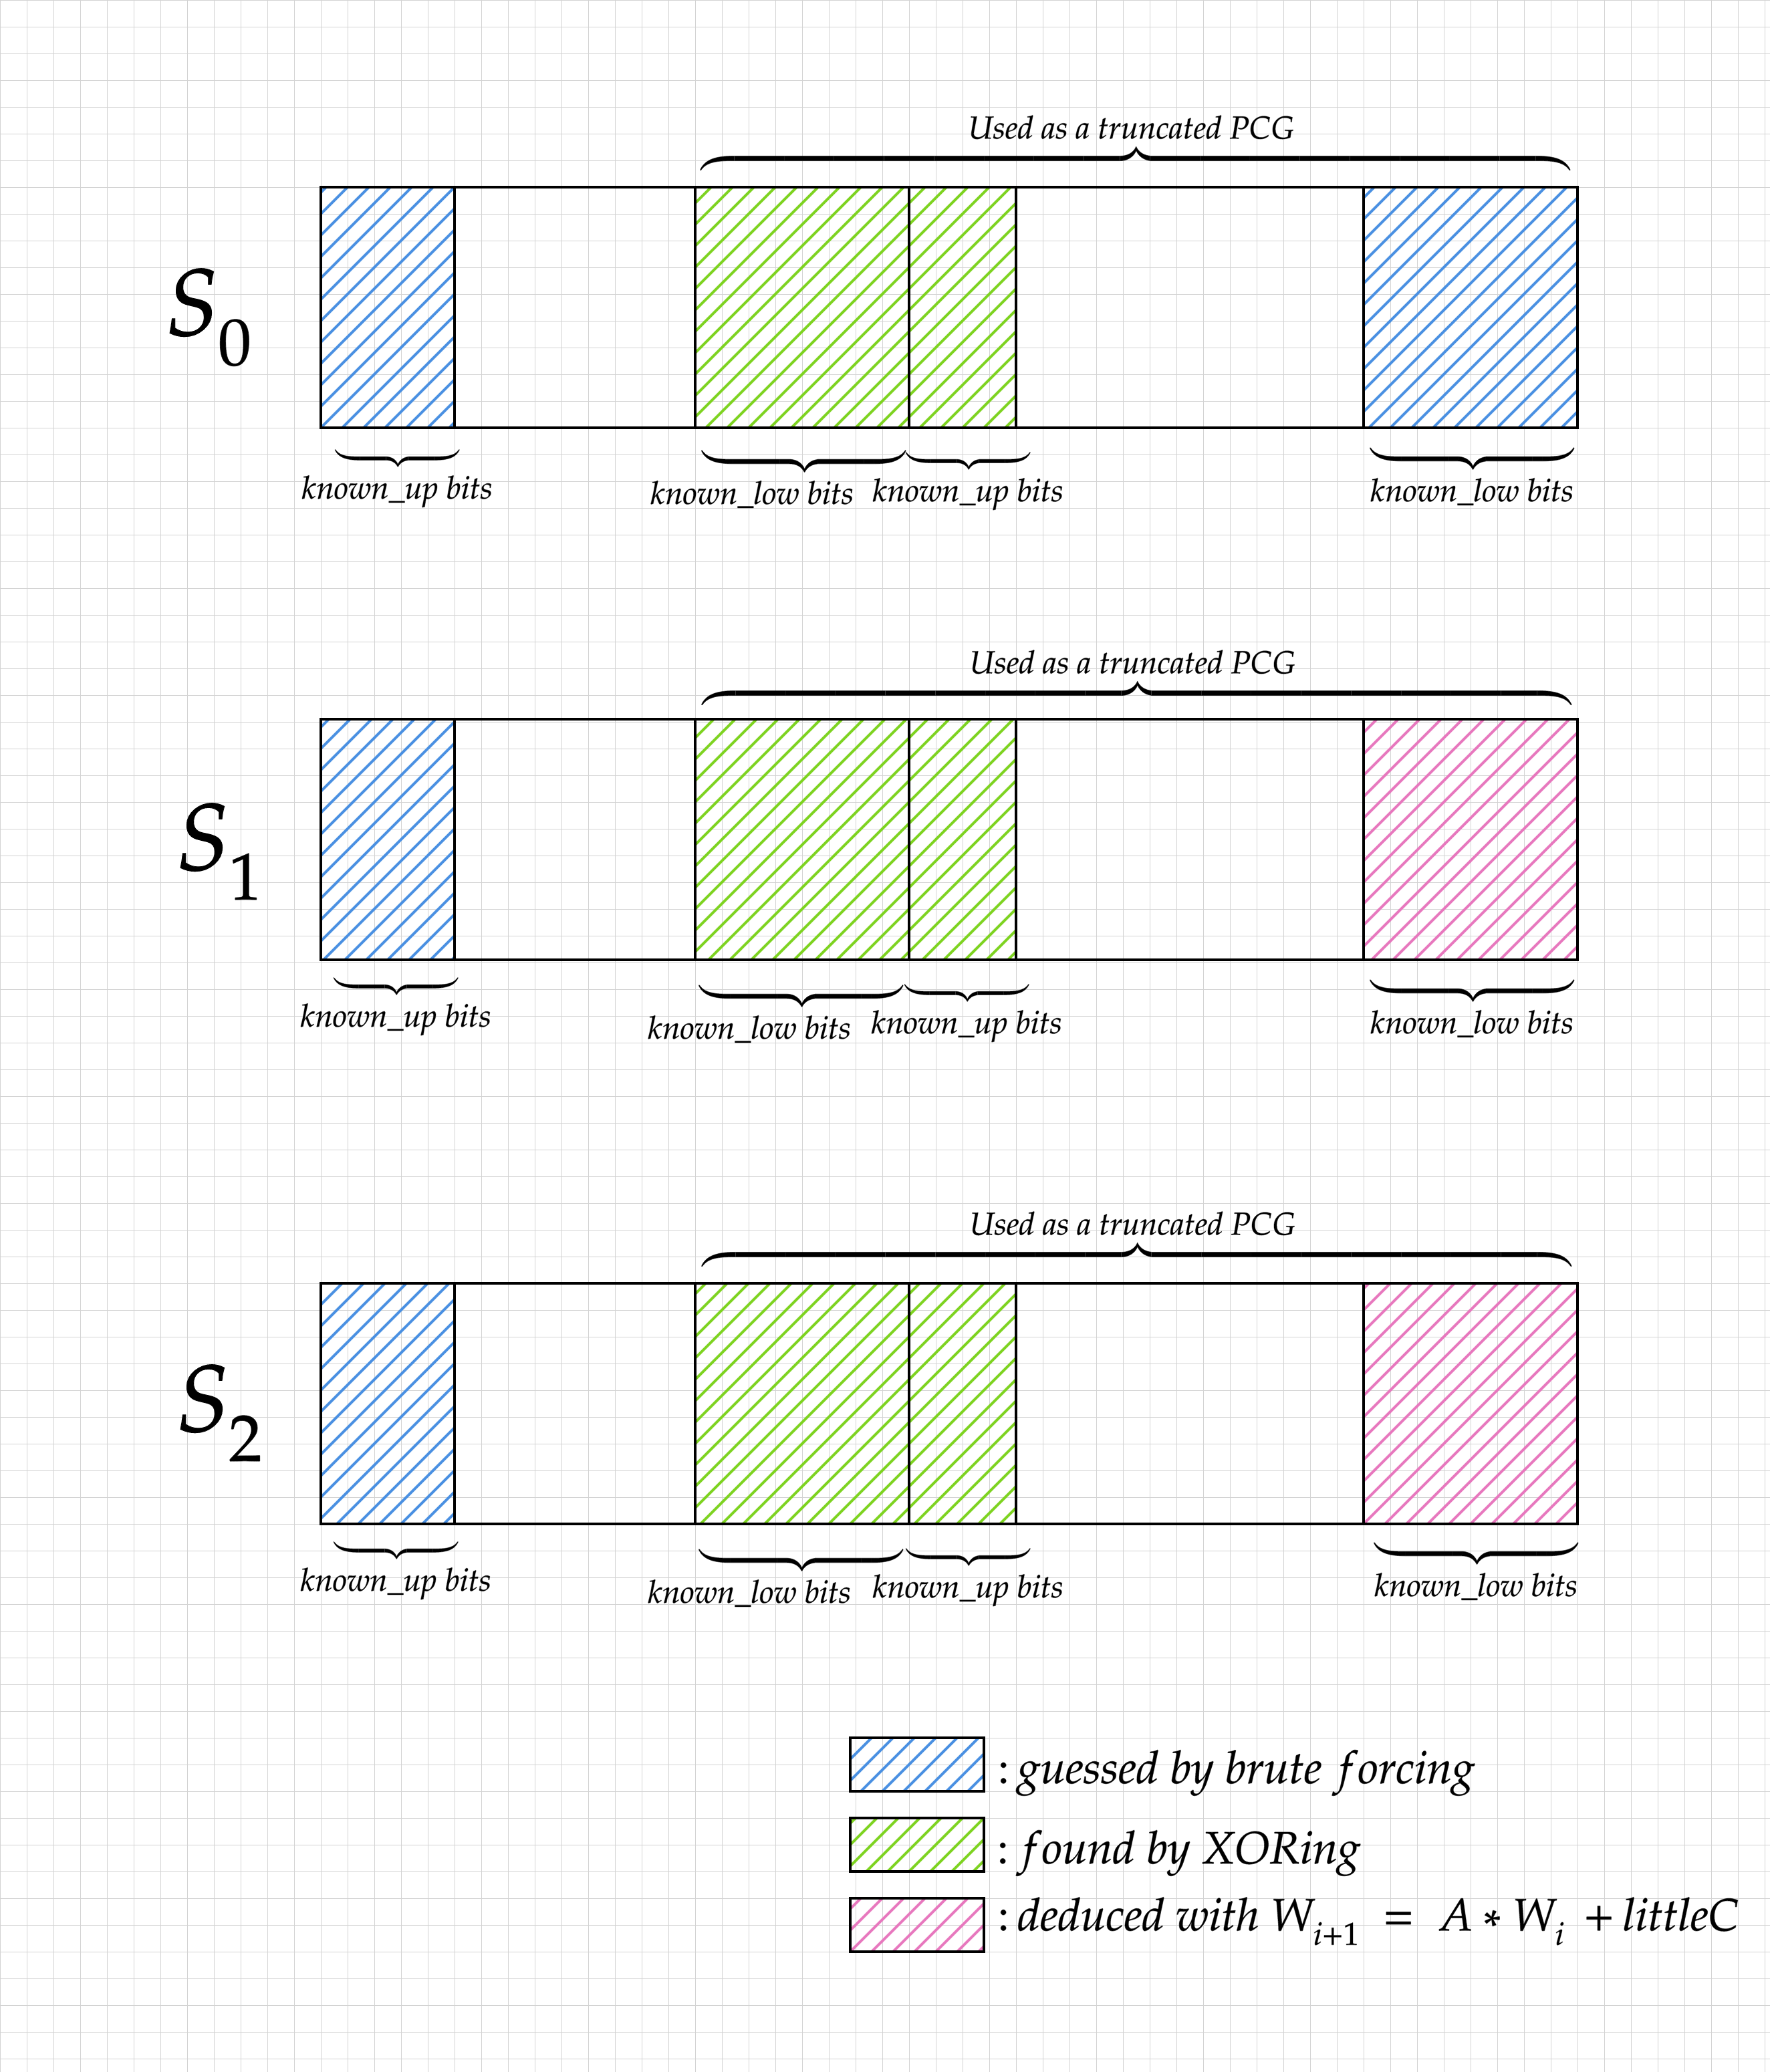
\includegraphics[width=0.70\linewidth]{pictures/deducingPCG128.png}
    \caption{PCG128 : Relevant bits of the outputs}
    \label{pcg128goodbits}
\end{figure}
that we can extract a lot of information by brute forcing certain well chosen bits. We defined $known\_up$ (respectively $known\_low$) the number of upper (respectively lower) bits searched by brute force.


\subsection{Reduction to a geometric sequence and validation of our values}

$C$ is known. We are looking for a geometric sequence $S'$ with which we can validate our brute-forced bits and extract $S_0$. Let $polC$ be the vector where $polC_i = \sum_{j=0}^{i} C \times A^j$ and $S'$ where $S'_i = S_i - polC_i$. We have :
\begin{align}
    S'_{i+1} &= S_{i+1} - polC_{i+1}\\
    S'_{i+1} &= A \times S_i + C - polC_{i+1}\\
    S'_{i+1} &= A \times S_i + C - (C + A \times C + ...+ A^{i} \times C)\\
    S'_{i+1} &= A \times (S'_i + polC_i) - A \times (C + ... + A^{i-1} \times C)\\
    S'_{i+1} &= A \times S'_i + A \times polC_i - A \times polC_i\\
    S'_{i+1} &= A \times S'_i
\end{align}

We have a convenient $S'$ that can be used in the algorithm presented in the previous section and, there exist a simple bijection between $S'$ and $S$. However, its important to notice that $S'$ will not be computed modulo $M = 2^k$ but modulo $N = 2^{k/2 + known\_low}$, because we are doing an comprehensive research of the middle bits of $S$ and not the upper ones (except for the 6 bits of $rot$). This is not a problem, because when we have the values of $X$, and $lowS$, we can always obtain $upS$ and ultimately $S$.\\



Using this bijection, we can validate if our chosen values are correct. Indeed, after finding $Z'$ through the LLL algorithm, we can compute $S'_0$ and $S'_1$ modulo $2^{k/2 + known\_low}$, then $S_0$ and $S_1$ modulo $2^{k/2 + known\_low}$, and finally $S_1$ and $S_0$. We verify if $S_1$ is coherent with $S_0$. If it is, then we have guessed the correct values for our generator, if not, we then consider this another value as our next test.

\newpage
 
\subsection{Pseudo-Algorithm}

\begin{algorithm}[h!]
\caption{Algorithm with known $C$}
\begin{algorithmic}
\REQUIRE $X$ the list of outputs
\STATE computation of the $LLL$ matrix
\STATE computation of $polC$
\FOR{ all $rot_i$ for $i$ in range($nbiter$) }
    \FOR{i in range($nbiter$)}
        \STATE \texttt{unrotate}($X_i$)
    \ENDFOR
    \FOR{all $W_0$}
        \STATE calculate the other $W_i$ with $W_0$ and $C$
        \STATE calculate $Y$ using $W_i\ \mathtt{XOR}\ X_i$ and $rot_i\ \mathtt{XOR}\ X_i$
        \STATE $W' = W - polC$ (we subtract only the corresponding bits of $C$)
        \STATE $Y' = Y - polC$
        \STATE calculation of $Z'$ due to LLL algorithm
        \IF{$2^{k/2-known\_up}>Y'>=2^{known\_low}$}
            \IF{$Z$ is correct}
                \STATE return the corresponding $S_0$
            \ENDIF
        \ENDIF
    \ENDFOR
\ENDFOR
\end{algorithmic}
\end{algorithm}
                
\subsection{Performance test results}
Our code is implemented in Sagemath. This choice was made because of the development advantages it offered: to be able to work with arbitrarily large integers and have access to a built-in LLL function.\\

The number of bits obtained by exhaustive research, as we have seen in the first section, is $nbiter \times known\_up + known\_low$. The most efficient way should be to only guess the lower bits ($known\_up = 0$). But we need the 6 bit value of $rot_i$ in our algorithm. So we kept $known\_up = 6$ and searched for the best equilibrium between $nbiter$ and $known\_low$. \\ 

Moreover, we also need this algorithm to be reliable. That is a concern because we know that there is a rounding error caused by an Euclidian Division. Depending on the error, it is possible that the algorithm doesn't find the correct $Z$ even if $Y$ and $W$ are correct (with $W$ the lower bits of $S$ and $Y$ the middle bits of $S$ found by \texttt{XOR}). \\

We tested the reliability and the efficiency of the algorithm. By trial and error, we ended up finding two interesting settings :
\begin{itemize}
    \item $known\_low = 16$ and $nbiter = 4$ : we have a $2^{40}$ brute-force algorithm. When supplying it with PCG128 outputs, the rate at which the algorithm detects it and obtains the correct $S_0$ is of 90\%.
    \item $known\_low = 15$ and $nbiter = 4$ : we have a $2^{39}$ brute-force algorithm. When supplying it with PCG128 outputs, the rate at which the algorithm detects it and obtains the correct $S_0$ is of 70\%.
\end{itemize}

In any case, if we supply a random output, the algorithm will detect this and will never return a false $S_0$. When not finding $S_0$, the default answer is to disqualify the input as a PCG data steam.\\

Unfortunately, we didn't get to run our entire solution in a real time environment, because with our personal equipment, and not fully optimized code, we estimated that it would have take more or less ten years to obtain an answer, which is obviously too long.
The local environment at the university didn't provide the right tools (SageMath), which complexified the development process of sharing the computation load between multiple computers. However, there are some methods and coding improvements to reduce the time needed, as we will discuss in the next section.

[insert here] attack predicting algo description.

\begin{theorem}
  The algorithm described above works with probability.... in time ...
\end{theorem}

\section{Predicting PCG with Unknown Increment}

[insert here] attack predicting algo description. Phase 1, Phase 2, Phase 3

\begin{theorem}
  The algorithm described above works with probability.... in time ...
\end{theorem}

\section{Implementation of the Predictor and Practical Results}

\section{Conclusion}

\bibliographystyle{alpha}
\bibliography{biblio}

%\appendix

\end{document}
